\documentclass[9pt,a4paper,]{extarticle}

\usepackage{f1000_styles}

\usepackage[pdfborder={0 0 0}]{hyperref}

\usepackage[numbers]{natbib}
\bibliographystyle{unsrtnat}


%% maxwidth is the original width if it is less than linewidth
%% otherwise use linewidth (to make sure the graphics do not exceed the margin)
\makeatletter
\def\maxwidth{ %
  \ifdim\Gin@nat@width>\linewidth
    \linewidth
  \else
    \Gin@nat@width
  \fi
}
\makeatother

\usepackage{color}
\usepackage{fancyvrb}
\newcommand{\VerbBar}{|}
\newcommand{\VERB}{\Verb[commandchars=\\\{\}]}
\DefineVerbatimEnvironment{Highlighting}{Verbatim}{commandchars=\\\{\}}
% Add ',fontsize=\small' for more characters per line
\usepackage{framed}
\definecolor{shadecolor}{RGB}{248,248,248}
\newenvironment{Shaded}{\begin{snugshade}}{\end{snugshade}}
\newcommand{\AlertTok}[1]{\textcolor[rgb]{0.94,0.16,0.16}{#1}}
\newcommand{\AnnotationTok}[1]{\textcolor[rgb]{0.56,0.35,0.01}{\textbf{\textit{#1}}}}
\newcommand{\AttributeTok}[1]{\textcolor[rgb]{0.77,0.63,0.00}{#1}}
\newcommand{\BaseNTok}[1]{\textcolor[rgb]{0.00,0.00,0.81}{#1}}
\newcommand{\BuiltInTok}[1]{#1}
\newcommand{\CharTok}[1]{\textcolor[rgb]{0.31,0.60,0.02}{#1}}
\newcommand{\CommentTok}[1]{\textcolor[rgb]{0.56,0.35,0.01}{\textit{#1}}}
\newcommand{\CommentVarTok}[1]{\textcolor[rgb]{0.56,0.35,0.01}{\textbf{\textit{#1}}}}
\newcommand{\ConstantTok}[1]{\textcolor[rgb]{0.00,0.00,0.00}{#1}}
\newcommand{\ControlFlowTok}[1]{\textcolor[rgb]{0.13,0.29,0.53}{\textbf{#1}}}
\newcommand{\DataTypeTok}[1]{\textcolor[rgb]{0.13,0.29,0.53}{#1}}
\newcommand{\DecValTok}[1]{\textcolor[rgb]{0.00,0.00,0.81}{#1}}
\newcommand{\DocumentationTok}[1]{\textcolor[rgb]{0.56,0.35,0.01}{\textbf{\textit{#1}}}}
\newcommand{\ErrorTok}[1]{\textcolor[rgb]{0.64,0.00,0.00}{\textbf{#1}}}
\newcommand{\ExtensionTok}[1]{#1}
\newcommand{\FloatTok}[1]{\textcolor[rgb]{0.00,0.00,0.81}{#1}}
\newcommand{\FunctionTok}[1]{\textcolor[rgb]{0.00,0.00,0.00}{#1}}
\newcommand{\ImportTok}[1]{#1}
\newcommand{\InformationTok}[1]{\textcolor[rgb]{0.56,0.35,0.01}{\textbf{\textit{#1}}}}
\newcommand{\KeywordTok}[1]{\textcolor[rgb]{0.13,0.29,0.53}{\textbf{#1}}}
\newcommand{\NormalTok}[1]{#1}
\newcommand{\OperatorTok}[1]{\textcolor[rgb]{0.81,0.36,0.00}{\textbf{#1}}}
\newcommand{\OtherTok}[1]{\textcolor[rgb]{0.56,0.35,0.01}{#1}}
\newcommand{\PreprocessorTok}[1]{\textcolor[rgb]{0.56,0.35,0.01}{\textit{#1}}}
\newcommand{\RegionMarkerTok}[1]{#1}
\newcommand{\SpecialCharTok}[1]{\textcolor[rgb]{0.00,0.00,0.00}{#1}}
\newcommand{\SpecialStringTok}[1]{\textcolor[rgb]{0.31,0.60,0.02}{#1}}
\newcommand{\StringTok}[1]{\textcolor[rgb]{0.31,0.60,0.02}{#1}}
\newcommand{\VariableTok}[1]{\textcolor[rgb]{0.00,0.00,0.00}{#1}}
\newcommand{\VerbatimStringTok}[1]{\textcolor[rgb]{0.31,0.60,0.02}{#1}}
\newcommand{\WarningTok}[1]{\textcolor[rgb]{0.56,0.35,0.01}{\textbf{\textit{#1}}}}

% disable code chunks background
%\renewenvironment{Shaded}{}{}

% disable section numbers
\setcounter{secnumdepth}{0}

%% added by MLS, this is not in the F1000 style by default %%

\hypersetup{unicode=true,
            pdftitle={target: An R Package to Predict Combined Function of Transcription Factors},
            pdfkeywords={transcription-factors; DNA-binding; gene-expression; r-package; bioconductor; workflow},
            pdfborder={0 0 0},
            breaklinks=true}

%% End added by MLS %%

\setlength{\parindent}{0pt}
\setlength{\parskip}{6pt plus 2pt minus 1pt}


\usepackage{soul}

\begin{document}
\pagestyle{front}

\title{target: An R Package to Predict Combined Function of Transcription Factors}

\author[1]{Mahmoud Ahmed}
\author[1]{Deok Ryong Kim}
\affil[1]{Department of Biochemistry and Convergence Medical Sciences and Institute of Health Sciences, Gyeongsang National University School of Medicine. Jinju, Korea}

\maketitle
\thispagestyle{front}

\begin{abstract}
Researchers use ChIP binding data to identify potential transcription factor binding sites. Similarly, they use gene expression data from sequencing or microarrays to quantify the effect of the factor overexpression or knockdown on its targets. Therefore, the integration of the binding and expression data can be used to improve the understanding of a transcription factor function. Here, we implemented the binding and expression target analysis (BETA) in an R/Bioconductor package. This algorithm ranks the targets based on the distances of their assigned peaks from the factor ChIP experiment and the signed statistics from gene expression profiling with factor perturbation. We further extend BETA to integrate two sets of data from two factors to predict their targets and their combined functions. In this article, we briefly describe the workings of the algorithm and provide a workflow with a real dataset for using it. The gene targets and the aggregate functions of transcription factors YY1 and YY2 in HeLa cells were identified. Using the same datasets, we identified the shared targets of the two factors, which were found to be, on average, more cooperatively regulated.
\end{abstract}

\section*{Keywords}
transcription-factors; DNA-binding; gene-expression; r-package; bioconductor; workflow


\clearpage
\pagestyle{main}

\textbf{R version}: R version 4.1.0 (2021-05-18)

\textbf{Bioconductor version}: 3.13

\hypertarget{introduction}{%
\section{Introduction}\label{introduction}}

The \hl{binding} of a transcription factor to a genomic region (e.g., gene promoter) can have the effect of inducing or repressing its expression \citet{Latchman2001}. The binding sites can be identified using ChIP experiments. High through-put ChIP experiments produce hundreds or thousands of binding sites for most factors \citet{Johnson2007a}. Therefore, methods to determine which of these sites are true \hl{binding sites} and whether they are functional or not are needed \citet{Ucar2009}. On the other hand, perturbing the transcription factor by over-expression or knockdown and measuring the gene expression changes provide valuable information on the function of the factor \citet{Tran2005}. Methods exist to integrate the binding data and the factor perturbation gene expression to predict the real target regions (e.g., genes) \citep{Subramanian2005, Wang2013b}. This article presents a workflow for using the target package to integrate binding and expression data to predict the shared targets and the combined function of two transcription factors.

To illustrate the utility of this workflow, we applied it to \hl{the} binding and expression data of the transcription factors YY1 and YY2. We asked whether the two factors cooperate or compete on their shared targets in HeLa cells.

\hypertarget{methods}{%
\section{Methods}\label{methods}}

\hypertarget{implementation}{%
\subsection{Implementation}\label{implementation}}

We developed an open-source R/Bioconductor package target to implement BETA for predicting direct transcription factor targets from binding and expression data. The details of the algorithm were described here \citet{Wang2013b}. In addition, our implementation extends BETA to apply for factor combinations (\citet{Ahmed2020}). Briefly, \hl{we identify the} factor potential binding sites by ChIP-sequencing and gene expression under factor perturbation by microarrays or sequencing. Next, \hl{we score the peaks based on their} distances to the transcription start sites. The sum of the scores of the individual peaks in a certain region of interest is the region's regulatory potential. \hl{The} signed statistics (fold-change or t-statistics) from the differential gene expression of the factor perturbation \hl{reflect} the factor \hl{effects}. The product of the ranks of the regulatory potential and the signed statistics is the final rank of the regions.

To predict the combined function of two factors, two sets of data are required. The overlapping peaks are the potential binding sites. The product of the two signed statistics is the factor function. When the two factors agree in the direction of the regulation of a region where they both bind, they could be said to cooperate on this region. When the sign is opposite, they could be said to regulate that region competitively.

The package leverages the Bioconductor data structures such as GRanges and DataFrame to provide fast and flexible computation on the data \citet{Huber2015}. Similar to the original python implementation, the input data are the identified peaks from the ChIP-Seq experiment and the expression data from RNA-Seq or microarrays perturbation experiment. The final output is the peaks associated with the factor binding and the predicted direct targets. We use the term ``peaks'' to refer to the GRanges object that contains the coordinates of the peaks. \hl{Likewise,} we use the term ``region'' to refer to a similar object that contains the information on the regions of interest; genes, transcripts, promoter regions, etc. In both cases, additional information on the ranges can be added to the object as metadata.

\hypertarget{operation}{%
\subsection{Operation}\label{operation}}

The algorithm was implemented in R (\textgreater= 3.6) and should run on any operating system. Libraries required for running the workflow are listed and loaded below. Alternatively, a docker image is available with R and the libraries installed on an Ubuntu image: \url{https://hub.docker.com/r/bcmslab/target_flow}.

\begin{Shaded}
\begin{Highlighting}[]
\CommentTok{\# load required libraries}
\FunctionTok{library}\NormalTok{(GenomicRanges)}
\FunctionTok{library}\NormalTok{(Biostrings)}
\FunctionTok{library}\NormalTok{(rtracklayer)}
\FunctionTok{library}\NormalTok{(TxDb.Hsapiens.UCSC.hg19.knownGene)}
\FunctionTok{library}\NormalTok{(BSgenome.Hsapiens.UCSC.hg19)}
\FunctionTok{library}\NormalTok{(org.Hs.eg.db)}
\FunctionTok{library}\NormalTok{(tidyverse)}
\FunctionTok{library}\NormalTok{(BCRANK)}
\FunctionTok{library}\NormalTok{(seqLogo)}
\FunctionTok{library}\NormalTok{(target)}
\end{Highlighting}
\end{Shaded}

\hypertarget{use-case}{%
\section{Use Case}\label{use-case}}

YY1 and YY2 belong to the same family of transcription factors. YY1 is a zinc finger protein that directs \hl{histone} deacetylase and acetyltransferases of the promoters of many genes. \hl{The protein also binds to the enhancer regions of many of its targets.} The binding of YY1 to the regulatory regions of genes results in the induction or repression of their expression. YY2 is a \hl{paralog} of YY1. Similarly, it is a zinc finger protein with both activation or repression functions on its targets. We will attempt to answer the following questions \hl{using the target analysis:} Do the two transcription factors share the same target genes? What are the consequences of the binding of each factor on its targets? If the two factors share binding sites, what is the function of the two factors \hl{binding} to these sites?

To answer these questions, we use publicly available datasets to model the binding and gene expression under the transcription factors perturbations (Table \ref{tab:datasets}). This dataset was obtained in the form of differential expression between the two conditions from \href{http://www.licpathway.net/KnockTF/index.html}{KnockTF} \citet{Feng2019}. The first dataset is gene expression profiling using microarrays of YY1/YY2 knockdown and control HeLa cells. \hl{Next,} the binding sites of the factors in HeLa cells were determined using two ChIP-Seq datasets. The ChIP peaks were \hl{acquired} in the form of bed files from \href{https://chip-atlas.org}{ChIP-Atlas} \citet{Oki2018}. Finally, we used the \hl{UCSC} hg19 human genome to extract the genomic annotations.

Briefly, we first prepared the three sources of data for the target analysis. Then we predict the specific targets for each individual factor. Third, we predict the combined function of the two factors on the shared target genes. Finally, we show an example of a motif analysis of the competitively and cooperatively regulated targets.

\begin{table}[htbp]
\caption{\label{tab:datasets} Expression and binding data of YY1 and YY2 in HeLa cells.}
\centering
\begin{tabledata}{@{}llll@{}}
\header GEO ID & Data Type & Design & Ref. \\
\row GSE14964 & Microarrays & YY\#-knockdown & \citet{Chen2010} \\
\row GSE31417 & ChIP-Seq & YY1 vs input & \citet{Michaud2013} \\
\row GSE96878 & ChIP-Seq & YY2 vs input & \citet{Wu2017d} \\
\end{tabledata}
\end{table}

\begin{Shaded}
\begin{Highlighting}[]
\ControlFlowTok{if}\NormalTok{(}\SpecialCharTok{!}\FunctionTok{file.exists}\NormalTok{(}\StringTok{\textquotesingle{}data.zip\textquotesingle{}}\NormalTok{)) \{}
  \CommentTok{\# download the manuscript data}
  \FunctionTok{download.file}\NormalTok{(}\StringTok{\textquotesingle{}https://ndownloader.figshare.com/articles/10918463/versions/1\textquotesingle{}}\NormalTok{,}
                \AttributeTok{destfile =} \StringTok{\textquotesingle{}data.zip\textquotesingle{}}\NormalTok{)}
  
  \CommentTok{\# decompress file}
  \FunctionTok{unzip}\NormalTok{(}\StringTok{\textquotesingle{}data.zip\textquotesingle{}}\NormalTok{, }\AttributeTok{exdir =} \StringTok{\textquotesingle{}data\textquotesingle{}}\NormalTok{)}
\NormalTok{\}}
\end{Highlighting}
\end{Shaded}

\hypertarget{preparing-the-binding-data}{%
\subsection{Preparing the binding data}\label{preparing-the-binding-data}}

The ChIP peaks were downloaded in the form of separate bed files for each factor. We first locate the files in the \texttt{data/} directory and load the files using \texttt{import.bed}. Then the data is transformed into a suitable format, \texttt{GRanges}. The resulting object, \texttt{peaks}, is a \texttt{list} of two \texttt{GRanges} items, one for each factor.

\begin{Shaded}
\begin{Highlighting}[]
\CommentTok{\# locate the peaks bed files}
\NormalTok{peak\_files }\OtherTok{\textless{}{-}} \FunctionTok{c}\NormalTok{(}\AttributeTok{YY1 =} \StringTok{\textquotesingle{}data/Oth.Utr.05.YY1.AllCell.bed\textquotesingle{}}\NormalTok{,}
                \AttributeTok{YY2 =} \StringTok{\textquotesingle{}data/Oth.Utr.05.YY2.AllCell.bed\textquotesingle{}}\NormalTok{)}

\CommentTok{\# load the peaks bed files as GRanges}
\NormalTok{peaks }\OtherTok{\textless{}{-}} \FunctionTok{map}\NormalTok{(peak\_files, }\SpecialCharTok{\textasciitilde{}}\FunctionTok{GRanges}\NormalTok{(}\FunctionTok{import.bed}\NormalTok{(.x)))}
\end{Highlighting}
\end{Shaded}

\hypertarget{preparing-the-expression-data}{%
\subsection{Preparing the expression data}\label{preparing-the-expression-data}}

The differential expression data were downloaded in tabular format. After locating the files in \texttt{data/}, we read the files using \texttt{read\_tsv} and select and rename the relevant columns. The resulting object, \texttt{express}, is a \texttt{list} of two \texttt{tibble} items.

\begin{Shaded}
\begin{Highlighting}[]
\CommentTok{\# locate the expression text files}
\NormalTok{expression\_files }\OtherTok{\textless{}{-}} \FunctionTok{c}\NormalTok{(}\AttributeTok{YY1 =} \StringTok{\textquotesingle{}data/DataSet\_01\_18.tsv\textquotesingle{}}\NormalTok{,}
                      \AttributeTok{YY2 =} \StringTok{\textquotesingle{}data/DataSet\_01\_19.tsv\textquotesingle{}}\NormalTok{)}

\CommentTok{\# load the expression text files}
\NormalTok{express }\OtherTok{\textless{}{-}} \FunctionTok{map}\NormalTok{(expression\_files,}
               \SpecialCharTok{\textasciitilde{}}\FunctionTok{read\_tsv}\NormalTok{(.x, }\AttributeTok{col\_names =} \ConstantTok{FALSE}\NormalTok{) }\SpecialCharTok{\%\textgreater{}\%}
\NormalTok{                 dplyr}\SpecialCharTok{::}\FunctionTok{select}\NormalTok{(}\DecValTok{2}\NormalTok{, }\DecValTok{3}\NormalTok{, }\DecValTok{7}\NormalTok{, }\DecValTok{9}\NormalTok{) }\SpecialCharTok{\%\textgreater{}\%} \CommentTok{\#9}
                 \FunctionTok{setNames}\NormalTok{(}\FunctionTok{c}\NormalTok{(}\StringTok{\textquotesingle{}tf\textquotesingle{}}\NormalTok{, }\StringTok{\textquotesingle{}gene\textquotesingle{}}\NormalTok{, }\StringTok{\textquotesingle{}fc\textquotesingle{}}\NormalTok{, }\StringTok{\textquotesingle{}pvalue\textquotesingle{}}\NormalTok{)) }\SpecialCharTok{\%\textgreater{}\%}
                 \FunctionTok{filter}\NormalTok{(tf }\SpecialCharTok{\%in\%} \FunctionTok{c}\NormalTok{(}\StringTok{\textquotesingle{}YY1\textquotesingle{}}\NormalTok{, }\StringTok{\textquotesingle{}YY2\textquotesingle{}}\NormalTok{)) }\SpecialCharTok{\%\textgreater{}\%}
                 \FunctionTok{na.omit}\NormalTok{())}
\end{Highlighting}
\end{Shaded}

The knockdown of either factor in HeLa cells seems to change the expression of many genes in either direction (Figure \ref{fig:foldchange}A\&B). Moreover, the changes resulting from the separate knockdown of the factors are correlated (Figure \ref{fig:foldchange}C). These observations suggest that many of the regulated genes are shared targets of the two factors, or they respond similarly to their perturbation of either factor.

\begin{Shaded}
\begin{Highlighting}[]
\CommentTok{\# Figure 1}
\FunctionTok{par}\NormalTok{(}\AttributeTok{mfrow =} \FunctionTok{c}\NormalTok{(}\DecValTok{1}\NormalTok{, }\DecValTok{3}\NormalTok{))}

\CommentTok{\# volcano plot of YY1 knockdown}
\FunctionTok{plot}\NormalTok{(express}\SpecialCharTok{$}\NormalTok{YY1}\SpecialCharTok{$}\NormalTok{fc, }
     \SpecialCharTok{{-}}\FunctionTok{log10}\NormalTok{(express}\SpecialCharTok{$}\NormalTok{YY1}\SpecialCharTok{$}\NormalTok{pvalue),}
     \AttributeTok{xlab =} \StringTok{\textquotesingle{}Fold{-}change (log\_2)\textquotesingle{}}\NormalTok{,}
     \AttributeTok{ylab =} \StringTok{\textquotesingle{}P{-}value ({-}log\_10)\textquotesingle{}}\NormalTok{,}
     \AttributeTok{xlim =} \FunctionTok{c}\NormalTok{(}\SpecialCharTok{{-}}\DecValTok{4}\NormalTok{, }\DecValTok{4}\NormalTok{), }\AttributeTok{ylim =} \FunctionTok{c}\NormalTok{(}\DecValTok{0}\NormalTok{, }\DecValTok{6}\NormalTok{))}
\FunctionTok{title}\NormalTok{(}\StringTok{\textquotesingle{}(A)\textquotesingle{}}\NormalTok{)}

\CommentTok{\# volcano plot of YY2 knockdown}
\FunctionTok{plot}\NormalTok{(express}\SpecialCharTok{$}\NormalTok{YY2}\SpecialCharTok{$}\NormalTok{fc, }
     \SpecialCharTok{{-}}\FunctionTok{log10}\NormalTok{(express}\SpecialCharTok{$}\NormalTok{YY2}\SpecialCharTok{$}\NormalTok{pvalue),}
     \AttributeTok{xlab =} \StringTok{\textquotesingle{}Fold{-}change (log\_2)\textquotesingle{}}\NormalTok{,}
     \AttributeTok{ylab =} \StringTok{\textquotesingle{}P{-}value ({-}log\_10)\textquotesingle{}}\NormalTok{,}
     \AttributeTok{xlim =} \FunctionTok{c}\NormalTok{(}\SpecialCharTok{{-}}\DecValTok{4}\NormalTok{, }\DecValTok{4}\NormalTok{), }\AttributeTok{ylim =} \FunctionTok{c}\NormalTok{(}\DecValTok{0}\NormalTok{, }\DecValTok{6}\NormalTok{))}
\FunctionTok{title}\NormalTok{(}\StringTok{\textquotesingle{}(B)\textquotesingle{}}\NormalTok{)}

\CommentTok{\# plot fold{-}change of YY1 and YY2}
\FunctionTok{plot}\NormalTok{(express}\SpecialCharTok{$}\NormalTok{YY1}\SpecialCharTok{$}\NormalTok{fc[}\FunctionTok{order}\NormalTok{(express}\SpecialCharTok{$}\NormalTok{YY1}\SpecialCharTok{$}\NormalTok{gene)],}
\NormalTok{     express}\SpecialCharTok{$}\NormalTok{YY2}\SpecialCharTok{$}\NormalTok{fc[}\FunctionTok{order}\NormalTok{(express}\SpecialCharTok{$}\NormalTok{YY2}\SpecialCharTok{$}\NormalTok{gene)],}
     \AttributeTok{xlab =} \StringTok{\textquotesingle{}YY1{-}knockdown (log\_2)\textquotesingle{}}\NormalTok{,}
     \AttributeTok{ylab =} \StringTok{\textquotesingle{}YY2{-}knockdown (log\_2)\textquotesingle{}}\NormalTok{,}
     \AttributeTok{xlim =} \FunctionTok{c}\NormalTok{(}\SpecialCharTok{{-}}\DecValTok{4}\NormalTok{, }\DecValTok{4}\NormalTok{), }\AttributeTok{ylim =} \FunctionTok{c}\NormalTok{(}\SpecialCharTok{{-}}\DecValTok{4}\NormalTok{, }\DecValTok{4}\NormalTok{))}
\FunctionTok{title}\NormalTok{(}\StringTok{\textquotesingle{}(C)\textquotesingle{}}\NormalTok{)}
\end{Highlighting}
\end{Shaded}

\begin{figure}

{\centering \includegraphics[width=1\linewidth]{targetFlow_files/figure-latex/foldchange-1} 

}

\caption{Differential expression between factor knockdown and control HeLa cells. Gene expression was compared between transcription factors knockdown and control HeLa cells. The fold-change and p-values of (A) YY1- and (B) YY2-knockdown are shown as volcano plots. (C) Scatter plot of the fold-change of the YY1- and YY2-knockdown.}\label{fig:foldchange}
\end{figure}

\hypertarget{preparing-genome-annotation}{%
\subsection{Preparing genome annotation}\label{preparing-genome-annotation}}

\texttt{express} \hl{records the} gene information using the gene Symbols. \hl{We} mapped \hl{the Symbols} to the \hl{Entrez IDs} before extracting the genomic coordinates. To do that, we use the \texttt{org.Hs.eg.db} to \hl{convert} between the identifiers. Next, we use the \texttt{TxDb.Hsapiens.UCSC.hg19.knownGene} to get the genomic coordinates for the transcripts and \hl{extend} them to 100kb upstream from the transcription start sites.

\begin{Shaded}
\begin{Highlighting}[]
\CommentTok{\# load genome data}
\NormalTok{symbol\_entrez }\OtherTok{\textless{}{-}}\NormalTok{ AnnotationDbi}\SpecialCharTok{::}\FunctionTok{select}\NormalTok{(org.Hs.eg.db,}
                        \FunctionTok{unique}\NormalTok{(}\FunctionTok{c}\NormalTok{(express}\SpecialCharTok{$}\NormalTok{YY1}\SpecialCharTok{$}\NormalTok{gene)),}
                        \StringTok{\textquotesingle{}ENTREZID\textquotesingle{}}\NormalTok{, }\StringTok{\textquotesingle{}SYMBOL\textquotesingle{}}\NormalTok{) }\SpecialCharTok{\%\textgreater{}\%}
  \FunctionTok{setNames}\NormalTok{(}\FunctionTok{c}\NormalTok{(}\StringTok{\textquotesingle{}gene\textquotesingle{}}\NormalTok{, }\StringTok{\textquotesingle{}gene\_id\textquotesingle{}}\NormalTok{))}

\CommentTok{\# format genome to join with express}
\NormalTok{genome }\OtherTok{\textless{}{-}} \FunctionTok{promoters}\NormalTok{(TxDb.Hsapiens.UCSC.hg19.knownGene,}
            \AttributeTok{upstream =} \DecValTok{100000}\NormalTok{,}
            \AttributeTok{columns =} \FunctionTok{c}\NormalTok{(}\StringTok{\textquotesingle{}tx\_id\textquotesingle{}}\NormalTok{, }\StringTok{\textquotesingle{}tx\_name\textquotesingle{}}\NormalTok{, }\StringTok{\textquotesingle{}gene\_id\textquotesingle{}}\NormalTok{)) }\SpecialCharTok{\%\textgreater{}\%}
  \FunctionTok{as\_tibble}\NormalTok{() }\SpecialCharTok{\%\textgreater{}\%} \FunctionTok{mutate}\NormalTok{(}\AttributeTok{gene\_id =} \FunctionTok{as.character}\NormalTok{(gene\_id))}
\end{Highlighting}
\end{Shaded}

The resulting object, \texttt{genome}, from the previous step is a \texttt{tibble} that shares the column \texttt{gene\_id} with the expression data \texttt{express}. Now the two objects can be merged. The merged object, \texttt{regions}, is similarly a \texttt{tibble} containing genome and expression information of all common genes.

\begin{Shaded}
\begin{Highlighting}[]
\CommentTok{\# make regions by merging the genome and express data}
\NormalTok{regions }\OtherTok{\textless{}{-}} \FunctionTok{map}\NormalTok{(express,}
               \SpecialCharTok{\textasciitilde{}}\FunctionTok{inner\_join}\NormalTok{(genome, symbol\_entrez) }\SpecialCharTok{\%\textgreater{}\%}
                 \FunctionTok{inner\_join}\NormalTok{(.x) }\SpecialCharTok{\%\textgreater{}\%}
                 \FunctionTok{makeGRangesFromDataFrame}\NormalTok{(}\AttributeTok{keep.extra.columns =} \ConstantTok{TRUE}\NormalTok{))}
\end{Highlighting}
\end{Shaded}

\hypertarget{predicting-gene-targets-of-individual-factors}{%
\subsection{Predicting gene targets of individual factors}\label{predicting-gene-targets-of-individual-factors}}

The standard target analysis \hl{identifies} associated peaks using \texttt{associated\_peaks} and direct targets using \texttt{direct\_targets}. The inputs for these functions are the objects \texttt{peaks} and \texttt{regions} from the previous steps in addition to the column names for regions \texttt{regions\_col} or the region and the statistics column \texttt{stats\_col}, which is the fold-change in this case. The resulting objects are \texttt{GRanges} for the identified peaks assigned to the regions, \texttt{ap}, or the ranked targets. Several columns are added to the metadata objects of the \texttt{GRanges} to save the \hl{output}.

\begin{Shaded}
\begin{Highlighting}[]
\CommentTok{\# get associated peaks}
\NormalTok{ap }\OtherTok{\textless{}{-}} \FunctionTok{map2}\NormalTok{(peaks, regions,}
           \SpecialCharTok{\textasciitilde{}}\FunctionTok{associated\_peaks}\NormalTok{(}\AttributeTok{peaks=}\NormalTok{.x,}
                             \AttributeTok{regions =}\NormalTok{ .y,}
                             \AttributeTok{regions\_col =} \StringTok{\textquotesingle{}tx\_id\textquotesingle{}}\NormalTok{))}

\CommentTok{\# get direct targets}
\NormalTok{dt }\OtherTok{\textless{}{-}} \FunctionTok{map2}\NormalTok{(peaks, regions,}
           \SpecialCharTok{\textasciitilde{}}\FunctionTok{direct\_targets}\NormalTok{(}\AttributeTok{peaks=}\NormalTok{.x,}
                           \AttributeTok{regions =}\NormalTok{ .y,}
                           \AttributeTok{regions\_col =} \StringTok{\textquotesingle{}tx\_id\textquotesingle{}}\NormalTok{,}
                           \AttributeTok{stats\_col =} \StringTok{\textquotesingle{}fc\textquotesingle{}}\NormalTok{))}
\end{Highlighting}
\end{Shaded}

To determine the dominant function of a factor, we divide the targets by the direction of the effect of \hl{factor} knockdown. \hl{We group the targets by the change in gene} expression (regulatory potential). We use the empirical distribution function (ECDF) to show the fraction of targets with a specified regulatory potential or less. Because \hl{we use} the ranks rather than the absolute value of the regulatory potential, the lower the \hl{rank}, the higher the potential. Then, \{we compare\} the groups of targets to each other or \hl{to} a theoretical distribution.

\begin{Shaded}
\begin{Highlighting}[]
\CommentTok{\# Figure 2}
\FunctionTok{par}\NormalTok{(}\AttributeTok{mfrow =} \FunctionTok{c}\NormalTok{(}\DecValTok{1}\NormalTok{, }\DecValTok{3}\NormalTok{))}

\CommentTok{\# plot distance by score of associate peaks}
\FunctionTok{plot}\NormalTok{(ap}\SpecialCharTok{$}\NormalTok{YY1}\SpecialCharTok{$}\NormalTok{distance, ap}\SpecialCharTok{$}\NormalTok{YY1}\SpecialCharTok{$}\NormalTok{peak\_score,}
     \AttributeTok{xlab =} \StringTok{\textquotesingle{}Distance\textquotesingle{}}\NormalTok{, }\AttributeTok{ylab =} \StringTok{\textquotesingle{}Peak Score\textquotesingle{}}\NormalTok{,}
     \AttributeTok{main =} \StringTok{\textquotesingle{}(A)\textquotesingle{}}\NormalTok{)}
\FunctionTok{points}\NormalTok{(ap}\SpecialCharTok{$}\NormalTok{YY2}\SpecialCharTok{$}\NormalTok{distance, ap}\SpecialCharTok{$}\NormalTok{YY2}\SpecialCharTok{$}\NormalTok{peak\_score)}

\CommentTok{\# make labels, colors and groups}
\NormalTok{labs }\OtherTok{\textless{}{-}} \FunctionTok{c}\NormalTok{(}\StringTok{\textquotesingle{}Down\textquotesingle{}}\NormalTok{, }\StringTok{\textquotesingle{}None\textquotesingle{}}\NormalTok{, }\StringTok{\textquotesingle{}Up\textquotesingle{}}\NormalTok{)}
\NormalTok{cols }\OtherTok{\textless{}{-}} \FunctionTok{c}\NormalTok{(}\StringTok{\textquotesingle{}green\textquotesingle{}}\NormalTok{, }\StringTok{\textquotesingle{}gray\textquotesingle{}}\NormalTok{, }\StringTok{\textquotesingle{}red\textquotesingle{}}\NormalTok{)}

\CommentTok{\# make three groups by quantiles      }
\NormalTok{groups }\OtherTok{\textless{}{-}} \FunctionTok{map}\NormalTok{(dt,}\SpecialCharTok{\textasciitilde{}}\NormalTok{\{}
  \FunctionTok{cut}\NormalTok{(.x}\SpecialCharTok{$}\NormalTok{stat, }\AttributeTok{breaks =} \DecValTok{3}\NormalTok{, }\AttributeTok{labels =}\NormalTok{ labs)}
\NormalTok{\})}

\CommentTok{\# plot the group functions}
\FunctionTok{pmap}\NormalTok{(}\FunctionTok{list}\NormalTok{(dt, groups, }\FunctionTok{c}\NormalTok{(}\StringTok{\textquotesingle{}(B)\textquotesingle{}}\NormalTok{, }\StringTok{\textquotesingle{}(C)\textquotesingle{}}\NormalTok{)), }\ControlFlowTok{function}\NormalTok{(x, y, z) \{}
      \FunctionTok{plot\_predictions}\NormalTok{(x}\SpecialCharTok{$}\NormalTok{score\_rank,}
                       \AttributeTok{group =}\NormalTok{ y, }\AttributeTok{colors =}\NormalTok{ cols, }\AttributeTok{labels =}\NormalTok{ labs,}
                       \AttributeTok{xlab =} \StringTok{\textquotesingle{}Regulatory Potential\textquotesingle{}}\NormalTok{, }\AttributeTok{ylab =} \StringTok{\textquotesingle{}ECDF\textquotesingle{}}\NormalTok{)}
      \FunctionTok{title}\NormalTok{(z)}
\NormalTok{    \})}
\end{Highlighting}
\end{Shaded}

\begin{figure}

{\centering 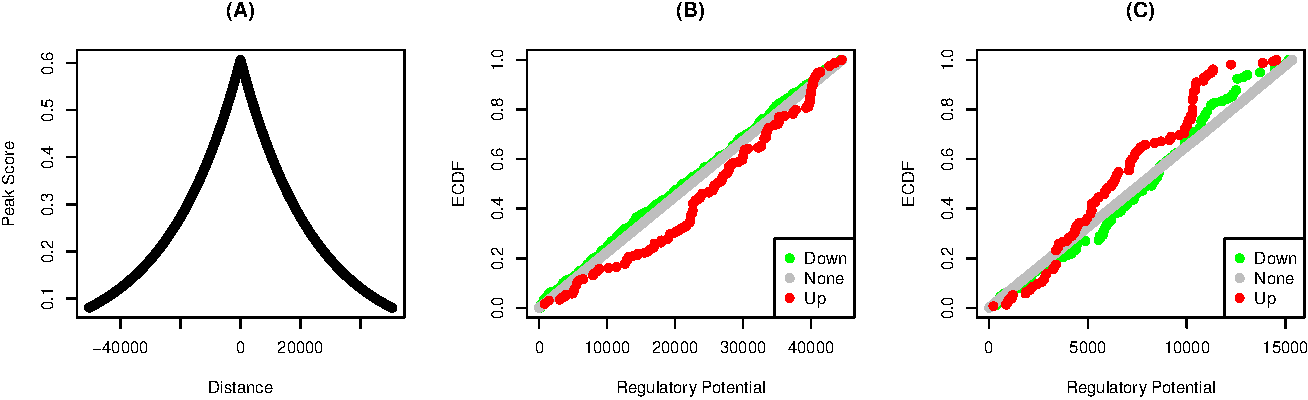
\includegraphics[width=1\linewidth]{targetFlow_files/figure-latex/functions-1} 

}

\caption{Predicted functions of YY1 and YY2 on their specific targets. Bindings peaks of the transcription factors in HeLa cells were determined using ChIP-Seq. Distances from the transcription start sites, and the transformed distances of the (A) YY1 and YY2 peaks are shown. The regulatory potential of each gene was calculated using target. Genes were grouped into up, none, or down-regulated based on the fold-change. The empirical cumulative distribution functions (ECDF) of the groups of (C) YY1 and (C) YY2 targets are shown at each regulatory potential rank.}\label{fig:functions}
\end{figure}

The scores of the individual peaks are a decreasing function of the distance from the transcription start sites---the closer the factor binding site from the start site, the \hl{higher} the score. The distribution of these scores is very similar for both factors (Figure \ref{fig:functions}A). The ECDF of the down-regulated of YY1 is higher than that of up-and none-regulated targets (Figure \ref{fig:functions}B). Therefore, the absence of YY1 on its targets results in aggregate in their downregulation. If indeed these are true targets, then we expect YY1 to induce their expression. The opposite is true for YY2, where more high-ranking targets are up-regulated by the factor knockdown (Figure \ref{fig:functions}C).

\begin{Shaded}
\begin{Highlighting}[]
\CommentTok{\# Table 2}
\CommentTok{\# test individual factor functions}
\FunctionTok{map2}\NormalTok{(dt, groups,}
     \SpecialCharTok{\textasciitilde{}}\FunctionTok{test\_predictions}\NormalTok{(.x}\SpecialCharTok{$}\NormalTok{rank,}
                       \AttributeTok{group =}\NormalTok{ .y,}
                       \AttributeTok{compare =} \FunctionTok{c}\NormalTok{(}\StringTok{\textquotesingle{}Down\textquotesingle{}}\NormalTok{, }\StringTok{\textquotesingle{}Up\textquotesingle{}}\NormalTok{)))}
\end{Highlighting}
\end{Shaded}

\begin{table}[htbp]
\caption{\label{tab:tests} Testing for statistical significance of the regulated gene groups.}
\centering
\begin{tabledata}{@{}lllll@{}}
\header Factor & Statistic & P.value & Method & Alternative \\
\row YY1 & 0.224 & 2.2e-16 & Two-sample KS test & two-sided \\
\row YY2 & 0.149 & 2.5e-15 & Two-sample KS test & two-sided \\
\end{tabledata}
\end{table}

To formally test these observations, we use the Kolmogorov-Smirnov (KS) test. \hl{First, we compare} the distributions of the two groups for equality. If one lies on either side of the other, then they must be drawn from different distributions. Here, we \hl{contrast} the up and down-regulated functions for both factors (Table \ref{tab:tests}). In both cases, the distributions of the two groups were significantly different from one another.

\hypertarget{predicting-the-shared-targets-of-two-factors}{%
\subsection{Predicting the shared targets of two factors}\label{predicting-the-shared-targets-of-two-factors}}

Using \texttt{target} to predict the shared target genes and the combined function of the two factors is a variation of the previous analysis. First, the shared/common peaks are generated using the overlap of their genomic coordinates, \texttt{subsetByOverlaps}. Second, Instead of one, two columns for the differential expression statistics, one for each factor is needed; these are supplied to the argument \texttt{stats\_col} in the same way. Here, \texttt{common\_peaks} and \texttt{both\_regions} are the main inputs for the analysis functions.

\begin{Shaded}
\begin{Highlighting}[]
\CommentTok{\# merge and name peaks}
\NormalTok{common\_peaks }\OtherTok{\textless{}{-}}\NormalTok{ GenomicRanges}\SpecialCharTok{::}\FunctionTok{reduce}\NormalTok{(}\FunctionTok{subsetByOverlaps}\NormalTok{(peaks}\SpecialCharTok{$}\NormalTok{YY1, peaks}\SpecialCharTok{$}\NormalTok{YY2))}
\NormalTok{common\_peaks}\SpecialCharTok{$}\NormalTok{name }\OtherTok{\textless{}{-}} \FunctionTok{paste0}\NormalTok{(}\StringTok{\textquotesingle{}common\_peak\_\textquotesingle{}}\NormalTok{, }\DecValTok{1}\SpecialCharTok{:}\FunctionTok{length}\NormalTok{(common\_peaks))}
\end{Highlighting}
\end{Shaded}

\begin{Shaded}
\begin{Highlighting}[]
\CommentTok{\# bind express tables into one}
\NormalTok{both\_express }\OtherTok{\textless{}{-}} \FunctionTok{bind\_rows}\NormalTok{(express) }\SpecialCharTok{\%\textgreater{}\%}
  \FunctionTok{nest}\NormalTok{(fc, pvalue, }\AttributeTok{.key =} \StringTok{\textquotesingle{}values\_col\textquotesingle{}}\NormalTok{) }\SpecialCharTok{\%\textgreater{}\%}
  \FunctionTok{spread}\NormalTok{(tf, values\_col) }\SpecialCharTok{\%\textgreater{}\%}
  \FunctionTok{unnest}\NormalTok{(YY1, YY2, }\AttributeTok{.sep =} \StringTok{\textquotesingle{}\_\textquotesingle{}}\NormalTok{)}

\CommentTok{\# make regions using genome and expression data of both factors}
\NormalTok{both\_regions }\OtherTok{\textless{}{-}} \FunctionTok{inner\_join}\NormalTok{(genome, symbol\_entrez) }\SpecialCharTok{\%\textgreater{}\%}
  \FunctionTok{inner\_join}\NormalTok{(both\_express) }\SpecialCharTok{\%\textgreater{}\%}
  \FunctionTok{makeGRangesFromDataFrame}\NormalTok{(}\AttributeTok{keep.extra.columns =} \ConstantTok{TRUE}\NormalTok{)}
\end{Highlighting}
\end{Shaded}

\begin{Shaded}
\begin{Highlighting}[]
\CommentTok{\# get associated peaks with both factors}
\NormalTok{common\_ap }\OtherTok{\textless{}{-}} \FunctionTok{associated\_peaks}\NormalTok{(}\AttributeTok{peaks =}\NormalTok{ common\_peaks,}
                              \AttributeTok{regions =}\NormalTok{ both\_regions,}
                              \AttributeTok{regions\_col =} \StringTok{\textquotesingle{}tx\_id\textquotesingle{}}\NormalTok{)}

\CommentTok{\# get direct targets of both factors}
\NormalTok{common\_dt }\OtherTok{\textless{}{-}} \FunctionTok{direct\_targets}\NormalTok{(}\AttributeTok{peaks =}\NormalTok{ common\_peaks,}
                            \AttributeTok{regions =}\NormalTok{ both\_regions,}
                            \AttributeTok{regions\_col =} \StringTok{\textquotesingle{}tx\_id\textquotesingle{}}\NormalTok{,}
                            \AttributeTok{stats\_col =} \FunctionTok{c}\NormalTok{(}\StringTok{\textquotesingle{}YY1\_fc\textquotesingle{}}\NormalTok{, }\StringTok{\textquotesingle{}YY2\_fc\textquotesingle{}}\NormalTok{))}
\end{Highlighting}
\end{Shaded}

The output, \texttt{associated\_peaks}, is \hl{similar to} before. \texttt{direct\_targets} is the same, but the \texttt{stat} and the \texttt{stat\_rank} \hl{columns} carry the product \hl{and the rank} of the two statistics provided in the previous step.

\hl{We can also visualize the output in a similar way}. The targets are divided into three groups based on the statistics product. When the two statistics agree in the sign, the product is positive. This means the knockdown of either transcription factor results in the same direction change in the target gene expression. Therefore, the two factors would cooperate if they bind to the same site on that gene. The reverse is true for targets with oppositely signed statistics. The two factors would be expected to compete on \hl{these targets} for inducing opposing changes in the expression.

\begin{Shaded}
\begin{Highlighting}[]
\CommentTok{\# Figure 3}
\FunctionTok{par}\NormalTok{(}\AttributeTok{mfrow =} \FunctionTok{c}\NormalTok{(}\DecValTok{1}\NormalTok{, }\DecValTok{2}\NormalTok{))}

\CommentTok{\# plot distiace by score for associated peaks}
\FunctionTok{plot}\NormalTok{(common\_ap}\SpecialCharTok{$}\NormalTok{distance,}
\NormalTok{     common\_ap}\SpecialCharTok{$}\NormalTok{peak\_score,}
     \AttributeTok{xlab =} \StringTok{\textquotesingle{}Distance\textquotesingle{}}\NormalTok{,}
     \AttributeTok{ylab =} \StringTok{\textquotesingle{}Peak Score\textquotesingle{}}\NormalTok{)}
\FunctionTok{title}\NormalTok{(}\StringTok{\textquotesingle{}(A)\textquotesingle{}}\NormalTok{)}

\CommentTok{\# make labels, colors and gorups}
\NormalTok{labs }\OtherTok{\textless{}{-}} \FunctionTok{c}\NormalTok{(}\StringTok{\textquotesingle{}Competitive\textquotesingle{}}\NormalTok{, }\StringTok{\textquotesingle{}None\textquotesingle{}}\NormalTok{, }\StringTok{\textquotesingle{}Cooperative\textquotesingle{}}\NormalTok{)}
\NormalTok{cols }\OtherTok{\textless{}{-}} \FunctionTok{c}\NormalTok{(}\StringTok{\textquotesingle{}green\textquotesingle{}}\NormalTok{, }\StringTok{\textquotesingle{}gray\textquotesingle{}}\NormalTok{, }\StringTok{\textquotesingle{}red\textquotesingle{}}\NormalTok{)}

\CommentTok{\# make three groups by quantiles      }
\NormalTok{common\_groups }\OtherTok{\textless{}{-}} \FunctionTok{cut}\NormalTok{(common\_dt}\SpecialCharTok{$}\NormalTok{stat,}
                     \AttributeTok{breaks =} \DecValTok{3}\NormalTok{,}
                     \AttributeTok{labels =}\NormalTok{ labs)}

\CommentTok{\# plot predicted function}
\FunctionTok{plot\_predictions}\NormalTok{(common\_dt}\SpecialCharTok{$}\NormalTok{score\_rank,}
                 \AttributeTok{group =}\NormalTok{ common\_groups,}
                 \AttributeTok{colors =}\NormalTok{ cols, }\AttributeTok{labels =}\NormalTok{ labs,}
                 \AttributeTok{xlab =} \StringTok{\textquotesingle{}Regulatory Interaction\textquotesingle{}}\NormalTok{, }\AttributeTok{ylab =} \StringTok{\textquotesingle{}ECDF\textquotesingle{}}\NormalTok{)}
\FunctionTok{title}\NormalTok{(}\StringTok{\textquotesingle{}(B)\textquotesingle{}}\NormalTok{)}
\end{Highlighting}
\end{Shaded}

\begin{figure}

{\centering \includegraphics[width=1\linewidth]{targetFlow_files/figure-latex/function-1} 

}

\caption{Predicted function of YY1 and YY2 on their shared targets. Shared bindings sites of YY1 and YY2 in HeLa cells were determined using the overlap of the individual factor ChIP-Seq peaks. (A) Distances from the transcription start sites, and the transformed distances of the shared peaks are shown. The regulatory interaction of each gene was calculated using target. Genes were grouped into cooperatively, none, or competitively regulated based on the product of the fold-changes from YY1- and YY2-knockdown. (B) The empirical cumulative distribution functions (ECDF) of the targets groups are shown at each regulatory potential rank.}\label{fig:function}
\end{figure}

The common peak distances and scores take the same shape (Figure \ref{fig:function}A). \hl{Furthermore,} the two factors seem to cooperate on more of the common target than any of the two other possibilities (Figure \ref{fig:function}B). This observation can be tested using the KS test. The curve of the cooperative targets lies above that of none and competitively regulated targets (Table \ref{tab:test}).

\begin{Shaded}
\begin{Highlighting}[]
\CommentTok{\# Table 3}
\CommentTok{\# test factors are cooperative}
\FunctionTok{test\_predictions}\NormalTok{(common\_dt}\SpecialCharTok{$}\NormalTok{score\_rank,}
                 \AttributeTok{group =}\NormalTok{ common\_groups,}
                 \AttributeTok{compare =} \FunctionTok{c}\NormalTok{(}\StringTok{\textquotesingle{}Cooperative\textquotesingle{}}\NormalTok{, }\StringTok{\textquotesingle{}None\textquotesingle{}}\NormalTok{),}
                 \AttributeTok{alternative =} \StringTok{\textquotesingle{}greater\textquotesingle{}}\NormalTok{)}

\CommentTok{\# test factors are more cooperative than competitive}
\FunctionTok{test\_predictions}\NormalTok{(common\_dt}\SpecialCharTok{$}\NormalTok{score\_rank,}
                 \AttributeTok{group =}\NormalTok{ common\_groups,}
                 \AttributeTok{compare =} \FunctionTok{c}\NormalTok{(}\StringTok{\textquotesingle{}Cooperative\textquotesingle{}}\NormalTok{, }\StringTok{\textquotesingle{}Competitive\textquotesingle{}}\NormalTok{),}
                 \AttributeTok{alternative =} \StringTok{\textquotesingle{}greater\textquotesingle{}}\NormalTok{)}
\end{Highlighting}
\end{Shaded}

\begin{table}[htbp]
\caption{\label{tab:test} Testing for statistical significance of combined functions of the two factors.}
\centering
\begin{tabledata}{@{}lllll@{}}
\header Compare & Statistic & P.value & Method & Alternative \\
\row Coop vs None & 0.168 & 1.5e-30 & KS test & The CDF of x lies above that of y \\
\row Coop vs Comp & 0.151 & 2.2e-16 & KS test & The CDF of x lies above that of y \\
\end{tabledata}
\end{table}

\hypertarget{binding-motif-analysis}{%
\subsection{Binding motif analysis}\label{binding-motif-analysis}}

\hl{The users can perform} any number of downstream analyses on the final output. For example, we could apply binding motif analysis to the groups of regulated targets. In this example, all the motif analysis itself is handled by the \texttt{BCRANK} package \citet{Ameur2009}. Here, we explain how to prepare the input from the shared peaks and target objects produced in the last step.

First, we extract the transcript IDs of the targets in their respective groups. Then the peaks assigned to these targets are ordered and sliced.

\begin{Shaded}
\begin{Highlighting}[]
\CommentTok{\# group peaks by their assigned targets}
\NormalTok{peak\_groups }\OtherTok{\textless{}{-}} \FunctionTok{split}\NormalTok{(common\_dt}\SpecialCharTok{$}\NormalTok{tx\_id, common\_groups)}

\CommentTok{\# reorder peaks and get top n peaks}
\NormalTok{peak\_groups }\OtherTok{\textless{}{-}} \FunctionTok{lapply}\NormalTok{(peak\_groups, }\ControlFlowTok{function}\NormalTok{(x) \{}
    \CommentTok{\# get peaks in x targets group}
\NormalTok{    p }\OtherTok{\textless{}{-}}\NormalTok{ common\_ap[common\_ap}\SpecialCharTok{$}\NormalTok{assigned\_region }\SpecialCharTok{\%in\%} \FunctionTok{unique}\NormalTok{(x)]}
    
    \CommentTok{\# order peaks by score}
\NormalTok{    p }\OtherTok{\textless{}{-}}\NormalTok{ p[}\FunctionTok{order}\NormalTok{(p}\SpecialCharTok{$}\NormalTok{peak\_score, }\AttributeTok{decreasing =} \ConstantTok{TRUE}\NormalTok{)]}
    
    \CommentTok{\# get n top peaks}
\NormalTok{    p[}\FunctionTok{seq\_len}\NormalTok{(}\FunctionTok{ifelse}\NormalTok{(}\FunctionTok{length}\NormalTok{(p) }\SpecialCharTok{\textgreater{}} \DecValTok{50}\NormalTok{, }\DecValTok{50}\NormalTok{, }\FunctionTok{length}\NormalTok{(p)))]}
\NormalTok{\})}
\end{Highlighting}
\end{Shaded}

The input for \texttt{bcrank} is a fasta file with the sequence of the regions to look for frequent motifs. We used the \texttt{BSgenome.Hsapiens.UCSC.hg19} to extract the sequences of the common peaks in the competitive and cooperative target groups. The sequences are first written to a temporary file and feed to the search function.

\begin{Shaded}
\begin{Highlighting}[]
\NormalTok{bcout }\OtherTok{\textless{}{-}} \FunctionTok{map}\NormalTok{(peak\_groups[}\FunctionTok{c}\NormalTok{(}\StringTok{\textquotesingle{}Competitive\textquotesingle{}}\NormalTok{, }\StringTok{\textquotesingle{}Cooperative\textquotesingle{}}\NormalTok{)], }\SpecialCharTok{\textasciitilde{}}\NormalTok{\{}
    \CommentTok{\# extract sequences of top peaks from the hg19 genome}
\NormalTok{    pseq }\OtherTok{\textless{}{-}} \FunctionTok{getSeq}\NormalTok{(BSgenome.Hsapiens.UCSC.hg19, }\AttributeTok{names =}\NormalTok{ .x)}
                 
    \CommentTok{\# write sequences to fasta file}
\NormalTok{    tmp\_fasta }\OtherTok{\textless{}{-}} \FunctionTok{tempfile}\NormalTok{()}
    \FunctionTok{writeXStringSet}\NormalTok{(pseq, tmp\_fasta)}
                 
    \CommentTok{\# set random see}
    \FunctionTok{set.seed}\NormalTok{(}\DecValTok{1234}\NormalTok{)}
                  
    \CommentTok{\# call bcrank with the fasta file}
    \FunctionTok{bcrank}\NormalTok{(tmp\_fasta, }\AttributeTok{silent =} \ConstantTok{TRUE}\NormalTok{)}
\NormalTok{\})}
\end{Highlighting}
\end{Shaded}

The sequences in the search path of the regions of interest are shown in (Figure \ref{fig:occurrences}). In the competitively regulated regions, one sequence was more frequent than all other sequences. By contrast, no sequence was uniquely frequent in the regions of cooperative targets.

\begin{Shaded}
\begin{Highlighting}[]
\CommentTok{\# Figure 4}
\FunctionTok{par}\NormalTok{(}\AttributeTok{mfrow =} \FunctionTok{c}\NormalTok{(}\DecValTok{1}\NormalTok{, }\DecValTok{2}\NormalTok{))}

\CommentTok{\# plot the occurrences of consensus sequesnce in the regions}
\FunctionTok{map2}\NormalTok{(bcout, }\FunctionTok{c}\NormalTok{(}\StringTok{\textquotesingle{}(A)\textquotesingle{}}\NormalTok{, }\StringTok{\textquotesingle{}(B)\textquotesingle{}}\NormalTok{), }\SpecialCharTok{\textasciitilde{}}\NormalTok{\{}
    \FunctionTok{plot}\NormalTok{(}\FunctionTok{toptable}\NormalTok{(.x, }\DecValTok{1}\NormalTok{))}
    \FunctionTok{title}\NormalTok{(.y)}
\NormalTok{\})}
\end{Highlighting}
\end{Shaded}

\begin{figure}

{\centering \includegraphics[width=1\linewidth]{targetFlow_files/figure-latex/occurrences-1} 

}

\caption{Occurrences of consensus sequences in the ranked regions. The number of occurances of the sequences in the search path in the regions of (A) competitively and (B) cooperatively regulated regions.}\label{fig:occurrences}
\end{figure}

The most frequent motifs in the two groups are shown as seq logos using the \texttt{seqLogo} package (Figure \ref{fig:motifs}).

\begin{Shaded}
\begin{Highlighting}[]
\CommentTok{\# Figure 5}
\CommentTok{\# plot the sequence of the predicted motifs}
\FunctionTok{map}\NormalTok{(bcout, }\FunctionTok{c}\NormalTok{(}\StringTok{\textquotesingle{}(A)\textquotesingle{}}\NormalTok{, }\StringTok{\textquotesingle{}(B)\textquotesingle{}}\NormalTok{), }\SpecialCharTok{\textasciitilde{}}\NormalTok{\{}
    \FunctionTok{seqLogo}\NormalTok{(}\FunctionTok{pwm}\NormalTok{(}\FunctionTok{toptable}\NormalTok{(.x, }\DecValTok{1}\NormalTok{)))}
    \FunctionTok{title}\NormalTok{(.y)}
\NormalTok{\})}
\end{Highlighting}
\end{Shaded}

\begin{figure}

{\centering \includegraphics[width=1\linewidth]{targetFlow_files/figure-latex/motifs-1} 

}

\caption{Predicted motifs of the cooperative and competitive binding sites. The position weight matrices of the most frequent motifs in the (A) competitively and (B) cooperatively regulated regions were calculated and shown as sequence logos. y-axis represents the information content at each position. The size of each letter represents the frequency in which the letter occurs at that position.}\label{fig:motifs}
\end{figure}

\hypertarget{summary}{%
\section{Summary}\label{summary}}

In this article, we present a workflow for predicting the direct targets of a transcription factor by integrating binding and expression data. The target package implements the BETA algorithm ranking gene targets based on the distances of the ChIP peaks of the transcription factor \hl{relative to the TSSs of the} genes and the differential expression of the factor perturbation. To predict the combined function of two factors, two sets of data are used to find the shared peaks and the \hl{rank} product of their differential expression \hl{statistics}.

\hypertarget{software-availability}{%
\section{Software availability}\label{software-availability}}

This section will be generated by the Editorial Office before publication. Authors are asked to provide some initial information to assist the Editorial Office, as detailed below.

\begin{enumerate}
\def\labelenumi{\arabic{enumi}.}
\item
  URL link to where the software can be downloaded from or used by a non-coder (AUTHOR TO PROVIDE; optional)
\item
  URL link to the author's version control system repository containing the source code: \url{https://github.com/MahShaaban/target}
\item
  Link to source code as at time of publication (\emph{F1000Research} TO GENERATE)
\item
  Link to archived source code as at time of publication (\emph{F1000Research} TO GENERATE)
\item
  Software license (GPL-3)
\end{enumerate}

\hypertarget{author-information}{%
\section{Author information}\label{author-information}}

MA. Convinced the idea and wrote the draft of the manuscript.
DK. Contributed to writing and revising the manuscript.

\hypertarget{competing-interests}{%
\section{Competing interests}\label{competing-interests}}

No competing interests were disclosed.

\hypertarget{grant-information}{%
\section{Grant information}\label{grant-information}}

This study was supported by the National Research Foundation of Korea (NRF) grant funded by the Ministry of Science and ICT (MSIT) of the Korea government {[}2015R1A5A2008833 and 2020R1A2C2011416{]}.

\hypertarget{acknowledgments}{%
\section{Acknowledgments}\label{acknowledgments}}

We thank all lab members for the discussion and comments on the early drafts of the article.

{\small\bibliography{references.bib}}

\end{document}
